% =============================================================================
% CS7980 Capstone paper — CONFIRMATORY UPDATE (supersedes the Week-12 WIP).
%
% Updated 2026-07-18 with the completed registered campaign + companions:
%   - Section VI rewritten as CONFIRMATORY RESULTS: H2 (specialization) NULL;
%     agentless F1-dominant (Holm p<.001); H-verify (V1 self-consistency
%     rescue) does NOT replicate; H-hetero-precision CONFIRMED (both
%     registered sub-claims; 89% vs 54% golden-match at depth 3).
%   - SWE-PRBench E2: coverage gain replicates, F1 four-way tie.
%   - Completeness re-audited with THREE judge families (definitional split
%     33-76%; pair-judge kappa=0.95 vs is-it-real kappa=0.23).
%   - Related Work: 2026 concurrent nulls (Pappu ICML'26, Self-MoA) +
%     Zietsman correlated-error positioning; refs [12]-[16] added.
%   - Threats/Conclusion reframed: generation axis null, verification axis
%     = cross-family corroboration.
%
% Numbers traceable to rap-review-research: phase2-results/phase3-stats-report
% .json, phase3-swe-report.json, hetero-confirmatory/phase3-hetero-stats-
% report.json (+ fp-completeness*/ caches). All replayable, zero LLM calls.
%
% TODOs before submission (search "TODO"):
%   (1) Verify author lists of refs [12]-[16] against arXiv.
%   (2) Confirm fig1_architectures.png is the final 4-panel diagram.
% =============================================================================

\documentclass[conference]{IEEEtran}
\IEEEoverridecommandlockouts

\usepackage{cite}
\usepackage{amsmath,amssymb,amsfonts}
\usepackage{graphicx}
\usepackage{booktabs}
\usepackage{textcomp}
\usepackage{xcolor}
\usepackage{url}

% indicator function that needs no extra package
\newcommand{\ind}{\mathbf{1}}

\begin{document}

\title{Evaluating Multi-Agent Communication Topologies\\
for Automated Code Review: A Pre-Registered Study}

\author{\IEEEauthorblockN{En-Ping Su, Tong Wu, Shiting Huang, Mengshan Li}
\IEEEauthorblockA{Khoury College of Computer Sciences\\
Northeastern University, Vancouver, Canada}}

\maketitle

% =============================================================================
\begin{abstract}
Large Language Models (LLMs) are increasingly used for automated code
review, and recent multi-agent systems suggest that dividing work among
specialized agents can improve reasoning on complex tasks. It remains
unclear, however, whether the \emph{communication topology} among
agents---not merely their presence, nor the extra compute they consume---
affects review quality, cost, and efficiency. This paper asks, under a
pre-registered and compute-matched design, how communication topology
affects the effectiveness and efficiency of automated code review. We compare four approaches under identical
conditions: an Agentless single-LLM baseline, a compute-matched
Generalists-3 control (the same generalist sampled three times and merged),
a Hierarchical Authority architecture, and a Decentralized Peer Consensus
architecture; the Generalists-3 control separates ``more compute'' from
``specialization,'' making our primary hypothesis testable. We have
implemented a modular platform that reviews the same immutable pull-request
snapshot with all four architectures through a shared import, review,
validation, storage, and evaluation pipeline backed by a production LLM
service, isolating topology as the only independent variable; the design,
hypotheses, sample sizes, and analysis plan were pre-registered and prompts
frozen before confirmatory data collection. Evaluation spans three
complementary datasets: Qodo PR-Review-Bench (objective ground truth),
SWE-PRBench (agreement with human reviewers), and an actively developed
full-stack data portal used as an industrial case study, and reports both
strict (file+line) and semantic (independent-judge) matching. The
registered confirmatory campaign is complete: 99 Qodo and 50 SWE-PRBench
PRs $\times$ four architectures $\times$ three runs, plus a pre-registered
cross-family companion (Kimi K2.5, GLM~5). The primary specialization
hypothesis is null---at matched compute, role specialists tie plain
samples on recall ($p{=}0.73$)---and no multi-agent arm approaches the
single-pass baseline on F1 (0.36--0.38 vs.\ 0.49, Holm $p{<}0.001$):
extra homogeneous agents buy recall (0.63 vs.\ 0.50) but drown it in
false positives at 3--9$\times$ the cost, and the self-consistency rescue
our pilot suggested does not replicate. The verification axis is
different: findings corroborated by ${\geq}2$ independent model families
reach precision 0.72 vs.\ 0.54 single-arm at equal-or-higher F1, and
findings all three families agree on are real 89\% of the time vs.\ 54\%
for one model repeating itself across three runs (gap CI $[0.29, 0.41]$;
judge-invariant, $\kappa{=}0.95$ across two independent pair judges). In
multi-agent code review, diversity pays on the verification axis, not the
generation axis.
\end{abstract}

\begin{IEEEkeywords}
Large Language Models, Multi-Agent Systems, Automated Code Review, Software
Engineering, Evaluation Methodology, LLM Verification.
\end{IEEEkeywords}

% =============================================================================
\section{Introduction}

Code review is a central quality-assurance practice: before code is merged,
reviewers examine pull requests (PRs) for functional defects, security
problems, maintainability issues, and architectural inconsistencies. It is
also time-consuming and hard to scale, especially for full-stack systems
spanning frontend, backend, databases, and deployment infrastructure. LLMs
can summarize changes, flag bugs, and recommend fixes, and multi-agent
frameworks such as ChatDev and MetaGPT suggest decomposing complex tasks
among specialized agents~\cite{chatdev,metagpt}.

Existing work, however, usually evaluates complete agent systems rather than
isolating the role of communication topology, and rarely separates the
benefit of \emph{communication} from the benefit of the additional
\emph{compute} that a multi-agent system spends. A centralized manager may
behave very differently from a decentralized group in which agents discuss
findings directly: centralized coordination may be faster and cheaper, while
decentralized discussion may catch more cross-component issues. But either
could simply be winning because it samples the model more times. We
therefore study whether the structure of agent communication---holding the
model, prompts, roles, and compute budget fixed---changes review outcomes:

\begin{quote}
\textbf{RQ:} How does the communication topology of a multi-agent system
affect the effectiveness and efficiency of automated code review?
\end{quote}

We refine this into three sub-questions:
\begin{itemize}
  \item \textbf{RQ1 (Effectiveness).} Does topology change defect-detection
  quality (precision, recall, localization) and agreement with human
  reviewers?
  \item \textbf{RQ2 (Efficiency).} How does topology affect latency, token
  cost, and coordination overhead (LLM calls, inter-agent messages)?
  \item \textbf{RQ3 (Complexity interaction).} Does the effect of topology
  depend on PR complexity, e.g., localized versus cross-component changes?
\end{itemize}

We compare four architectures arranged as a ladder that changes one variable
per rung: \emph{Agentless} $\rightarrow$ \emph{Generalists-3} (+compute)
$\rightarrow$ \emph{Hierarchical Authority} (+specialization) $\rightarrow$
\emph{Decentralized Peer Consensus} (+peer communication). Agentless is a
strong single-LLM baseline, since simple non-agent pipelines can be
competitive on software-engineering tasks~\cite{agentless}. Generalists-3
runs the identical generalist prompt three times in parallel and merges the
results with the shared synthesizer: it holds the sampling budget equal to
the multi-agent arms but adds no roles and no communication, so it is the
compute-matched control that makes the primary (specialization) hypothesis
testable. Hierarchical and Consensus share specialist roles but differ in
how agents communicate.

Our contributions are:
\begin{itemize}
  \item A controlled design---pre-registered, with prompts frozen before
  confirmatory data collection---and an implemented, reproducible platform
  in which review architecture is the only independent variable, including a
  compute-matched generalist control.
  \item A three-dataset evaluation framework combining objective benchmark
  correctness, human-reviewer agreement, and an industrial case study, with
  both strict and semantic matching.
  \item An industrial verification methodology that corroborates findings
  without authoritative ground truth.
  \item Confirmatory results: a pre-registered null for role
  specialization and for homogeneous multi-agent F1 gains, a confirmatory
  refutation of our own pilot's self-consistency rescue, and a confirmed
  cross-family corroboration hypothesis---agreement between independent
  model families is a quantified, judge-invariant precision instrument
  (89\% vs.\ 54\% at full agreement)---plus a three-judge audit showing
  benchmark ground truth is materially incomplete.
\end{itemize}

% =============================================================================
\section{Related Work}

\subsection{LLM-Based Software Engineering}
LLMs have been applied to code generation, program repair, bug localization,
and test generation. SWE-bench benchmarks real GitHub issues and PRs and
shows the difficulty of resolving realistic problems with language
models~\cite{swebench}. Agentless challenges the assumption that complex
agent systems are always necessary, using a simple localize--repair--validate
pipeline~\cite{agentless}; its strong performance makes it an essential
baseline for judging whether multi-agent communication adds measurable
value.

\subsection{Multi-Agent Software Engineering}
Multi-agent systems assign roles to multiple LLM agents. ChatDev models
development as communication among design, coding, and testing
agents~\cite{chatdev}; MetaGPT adds structured workflows and role-based
collaboration to reduce inconsistency~\cite{metagpt}. Surveys argue the area
is promising but under-evaluated empirically~\cite{survey}, and other work
finds that agent systems fail through coordination overhead, cascading
errors, and weak verification~\cite{whyfail}. These failure modes are
precisely properties of communication structure, motivating our controlled
comparison of topologies rather than of whole systems. Concurrent work
sharpens the negative case: Pappu et al.\ show LLM teams underperform
their strongest member by up to 41\% through ``integrative
compromise''---averaging expert and non-expert views rather than
weighting expertise~\cite{pappu}---and Li et al.\ find that mixing
different LLMs rarely beats self-ensembling the best single model
(Self-MoA)~\cite{selfmoa}. Our compute-matched, pre-registered design
tests these dynamics in code review specifically; our confirmatory nulls
replicate them under a frozen-model discipline, and our cross-family
result locates where mixing \emph{does} pay.

\subsection{Evaluation Without Ground Truth}
Objective benchmarks require labeled defects, which real industrial
repositories rarely provide. Using a separate LLM as an impartial judge is
an increasingly common way to assess outputs at scale~\cite{llmjudge}. We
adopt LLM-as-a-judge as one corroboration signal---not a source of ground
truth---and combine it with cross-architecture agreement and conventional
static analysis to triangulate the credibility of findings on a live
repository.

\subsection{Verifying LLM Outputs}
A parallel line of work asks not how to \emph{generate} candidate outputs
but how to \emph{verify} them. Cobbe et al.\ show that a trained verifier can
outperform a much larger generator by re-ranking sampled
solutions~\cite{cobbe}. For LLM-as-a-judge specifically, Verga et al.\ find
that a panel of smaller diverse judges beats a single large
judge~\cite{verga}, while Panickssery et al.\ document a self-preference
bias in which evaluators favor their own generations~\cite{panickssery}---
directly motivating our non-circular design in which generator, matching
judge, and verifier are three different model families. Kwok et al.\ frame
verification as a general-purpose capability with three scaling axes---
scoring granularity, repeated evaluation, and criteria
decomposition~\cite{kwok}---the structure our strongest verifier (V3 below)
adapts. Closest to our confirmed hypothesis, Zietsman conjectures a
\emph{correlated-error} failure mode for AI code review---same-family
generator and reviewer share blind spots, so ``combining does not reduce
error, it consolidates it''---and contrasts same- vs.\ cross-family
reviewers on a small contrived corpus, self-described as directional and
unpowered~\cite{zietsman}. We provide what that argument lacks: a
pre-registered, statistically powered test against an external
injected-defect ground truth, operationalizing cross-family agreement as
a precision instrument (Section~\ref{sec:hetero}).

% =============================================================================
\section{Research Design}

\subsection{Variables}
\label{sec:variables}
The independent variable is communication topology across four
architectures: (1)~\emph{Agentless}: one LLM reviews the PR without agent
communication; (2)~\emph{Generalists-3}: the same generalist prompt sampled
three times in parallel and merged by the shared synthesizer---no roles, no
communication---serving as the compute-matched control; (3)~\emph{Hierarchical
Authority}: a manager assigns work to specialists and synthesizes their
findings; (4)~\emph{Decentralized Peer Consensus}: specialists review
independently, exchange findings, and vote to converge. Controlled variables
(model, prompts, roles, sampling budget, PR snapshot) are held fixed;
dependent variables capture effectiveness and efficiency (Table~\ref{tab:vars}).

\begin{table}[t]
\caption{Research Variables}
\label{tab:vars}
\centering
\begin{tabular}{ll}
\toprule
Type & Description \\
\midrule
Independent  & Communication topology (4 architectures) \\
Controlled   & Model, prompts, roles, sampling budget, PR snapshot \\
Effectiveness& Precision, recall, F1, localization; corroboration \\
Efficiency   & Latency, token cost, LLM calls, message count \\
\bottomrule
\end{tabular}
\end{table}

\subsection{Hypotheses}
The design, hypotheses, sample sizes, and analysis plan were pre-registered
on OSF (embargoed) and prompts frozen (tag \texttt{prompt-freeze-v1}) before
any confirmatory data collection. The registered contrasts are:

\begin{itemize}
  \item \textbf{H-specialization (primary).} Role-specialized teams
  (Hierarchical, Consensus) outperform the compute-matched Generalists-3
  control on defect-detection quality (RQ1). This is the confirmatory
  hypothesis; the Generalists-3 control is what makes it distinguishable
  from a mere compute effect.
  \item \textbf{H-compute (secondary).} Generalists-3 outperforms Agentless,
  isolating the value of additional sampling independent of structure (RQ1).
  \item \textbf{H-communication (secondary).} Peer communication (Consensus)
  outperforms coordinator-mediated aggregation (Hierarchical), especially on
  recall for cross-component PRs (RQ1, RQ3).
  \item \textbf{H-efficiency (secondary).} Latency, token cost, and
  coordination overhead rise monotonically along the ladder Agentless
  $\rightarrow$ Generalists-3 $\rightarrow$ Hierarchical $\rightarrow$
  Consensus (RQ2).
  \item \textbf{H-complexity (secondary).} The effect of topology grows with
  PR complexity (RQ3).
\end{itemize}

Two secondary confirmatory hypotheses were added by a pre-data OSF
amendment (submitted before any confirmatory collection), motivated by the
exploratory pilots: \textbf{H-verify}---a self-consistency filter (keep
findings recurring in ${\geq}2$ of 3 runs) lifts each multi-agent arm's
semantic F1 to within 0.02 of the Agentless baseline; and
\textbf{H-hetero-precision}---findings corroborated by ${\geq}2$ of three
independent model families \{Claude Haiku~4.5, Kimi K2.5, GLM~5\} achieve
precision ${\geq}10$ points above the mean single-arm precision at
equal-or-higher F1, and the golden-match rate of findings agreed by all
three families exceeds the frozen model's own three-run recurrence by
${\geq}10$ points, claimed only if the CI excludes a ${<}5$-point gap. The
companion families were selected by a pre-specified parity gate (single-arm
semantic F1 ${\geq}0.85\times$ the best family's), and the ${\leq}21$ pilot
PRs used for that screening are excluded from the H-hetero-precision test
set. A model-scale arm (Claude Sonnet~4.5 replacing Haiku~4.5) is
exploratory, used to check that the architecture ordering is model-robust
rather than an artifact of a single generator.

% =============================================================================
\section{Platform and Methodology}

\subsection{Experimental Platform}
We implemented a modular platform that drives every architecture through the
same pipeline: PR import produces an immutable snapshot; the architecture
under test reviews that snapshot; a validation stage normalizes raw model
output into structured findings; results are stored; and an evaluation
engine computes metrics. A campaign runner imports each PR once and reviews
the shared snapshot with all four architectures, so topology is the only
variable (fairness policy). All arms run \textbf{Claude Haiku~4.5} as the
frozen system under test (with \textbf{Claude Sonnet~4.5} as a robustness
arm), with temperature and prompts frozen; reviews run on Amazon Bedrock.
Semantic matching and verification use non-Anthropic model
families---\textbf{Llama 3.3~70B} as the finding$\to$ground-truth judge,
\textbf{Amazon Nova~Pro} as the cross-family finding$\leftrightarrow$finding
pair judge, and \textbf{DeepSeek~V3.2} as verifier and second judge---so no
model family scores its own family's output, and each judging role is
cross-checked by a second independent family.

\subsection{Architectures}
Figure~\ref{fig:architectures} contrasts the four architectures. Agentless
reviews the diff in a single pass. Generalists-3 runs that same generalist
review three times in parallel and merges the outputs through the shared
synthesizer, matching the multi-agent sampling budget without adding roles
or communication. Hierarchical Authority has a coordinator (manager) direct
frontend, backend, and database specialists, then deterministically merges
their findings. Decentralized Peer Consensus uses the same specialists,
which first review independently, then exchange findings and vote to reach a
shared set. The multi-agent architectures share specialist implementations
and prompts, differing only in coordination and message flow.

\begin{figure*}[t]
\centering
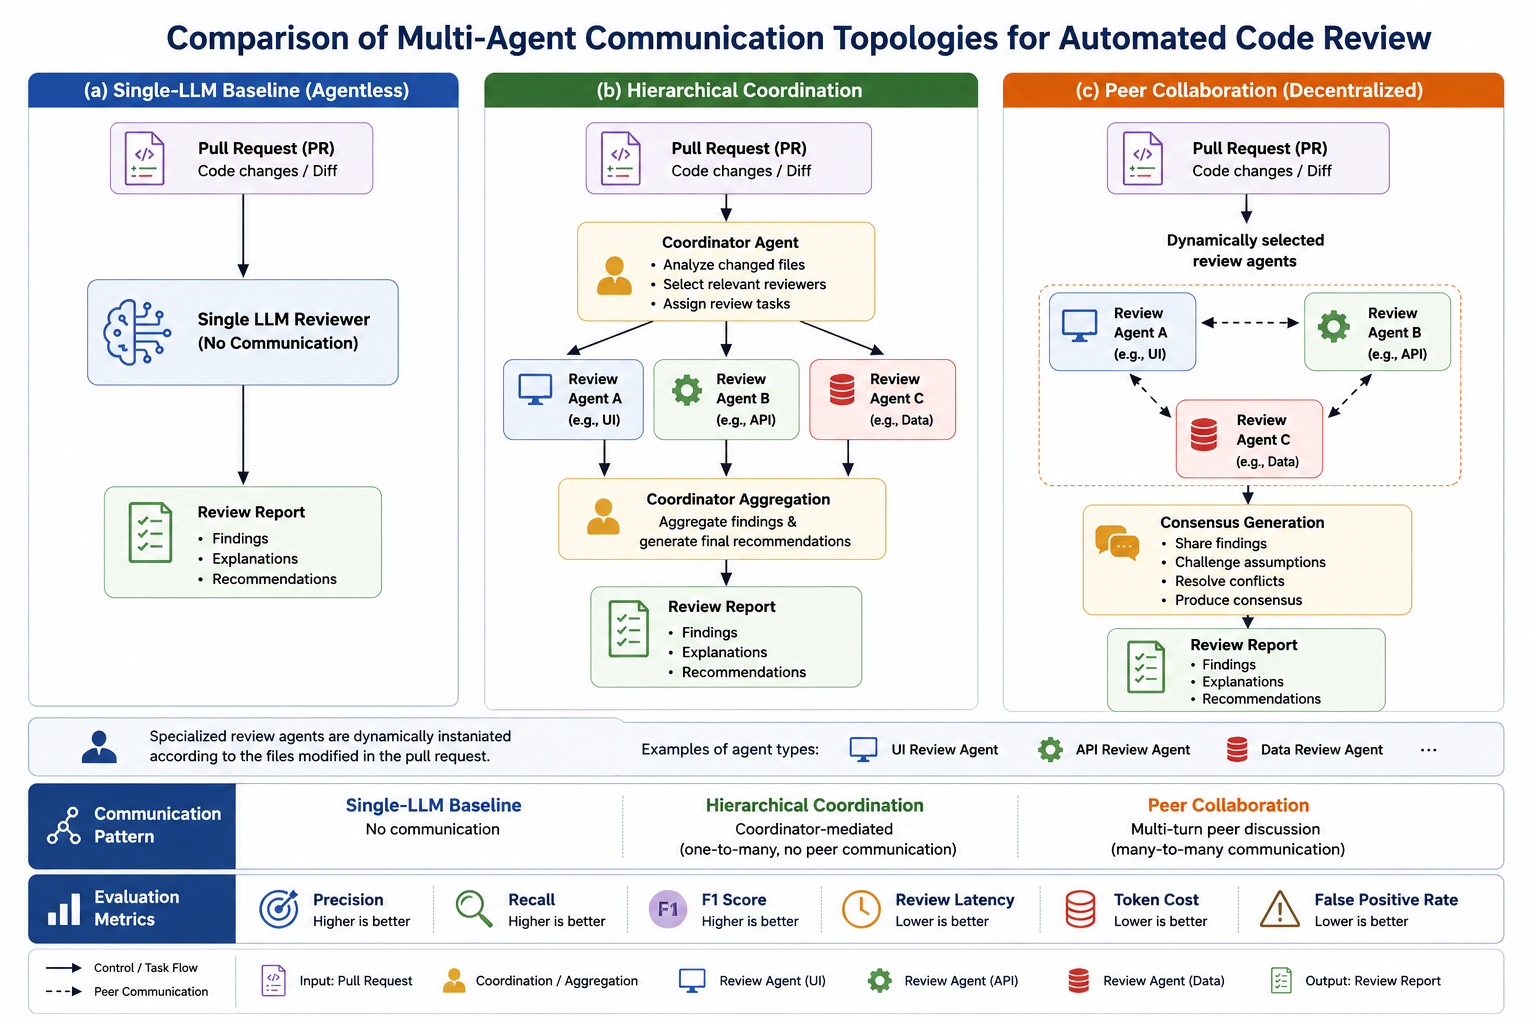
\includegraphics[width=\textwidth]{fig1_architectures.png}
\caption{The three communication topologies compared. (a)~\emph{Agentless}:
a single LLM reviews the pull request with no agent communication.
(b)~\emph{Hierarchical Authority}: a coordinator assigns the diff to
specialist agents (e.g., UI, API, data) and aggregates their findings---a
one-to-many, coordinator-mediated pattern with no peer communication.
(c)~\emph{Decentralized Peer Consensus}: dynamically selected specialists
review independently and then discuss directly (many-to-many) to resolve
conflicts and produce a consensus report. Solid arrows denote control/task
flow; dashed arrows denote peer communication. The compute-matched
\emph{Generalists-3} control (Section~\ref{sec:variables}) is Agentless
sampled three times in parallel and merged---no roles, no communication---so
it introduces no new communication topology and is described in the text
rather than shown as a separate panel.}
\label{fig:architectures}
\end{figure*}

\subsection{Datasets}
Three datasets provide complementary evidence: \emph{Qodo PR-Review-Bench}
(PRs with injected defects and explicit ground truth $\rightarrow$
precision, recall, F1, localization); \emph{SWE-PRBench} (real PRs with
human review comments, interpreted as agreement with reviewers rather than
absolute correctness); and an \emph{industrial case study}---an actively
developed full-stack data portal (React frontend, backend APIs, database
logic, authentication, cloud deployment)---reviewed on real PRs for
ecological validity but without authoritative ground truth.

\subsection{Evaluation Metrics}
Metrics are read according to the evidence each dataset offers
(Table~\ref{tab:metrics}). For the industrial case study, correctness cannot
be measured directly, so we do not report precision/recall/F1. Instead,
\emph{industrial verification} corroborates findings via: (i)~Cross-Architecture
Agreement---the fraction of an architecture's findings independently found by
another architecture on the same PR (matched on file, line, category, and
title similarity); (ii)~Static-Analysis Agreement---the fraction coinciding
with issues from conventional static-analysis tools; (iii)~LLM-Judge
Validation---the fraction a separate, impartial LLM classifies as valid given
the diff; (iv)~Later-Fix Rate---the fraction whose location is modified in
later commits; and (v)~Evidence Score, a supporting heuristic over severity,
confidence, and finding volume that reflects review strength, not
correctness. Operational metrics (latency, tokens, cost, LLM calls,
messages) are collected identically across all datasets.

Formally, let $F$ be an architecture's validated findings on a PR and $A_x$
the findings of architecture $x$. Writing $m(f, S) = 1$ when a finding $f$
matches some element of set $S$ (same file, a small line window, and
matching category or title), the corroboration signals are
\begin{align}
\mathrm{CAA}_x &= \frac{1}{|A_x|}\sum_{f \in A_x}
   \ind\!\left[\exists\, y \neq x : m(f, A_y)\right], \\
\mathrm{SAA} &= \frac{1}{|F|}\sum_{f \in F}
   \ind\!\left[m(f, S_{\text{static}})\right], \\
\mathrm{LJV} &= \frac{1}{|F|}\,\big|\{f \in F : \mathrm{judge}(f) = \text{valid}\}\big|, \\
\mathrm{LFR} &= \frac{1}{|F|}\,\big|\{f \in F : \mathrm{loc}(f)\ \text{changed later}\}\big|,
\end{align}
where $S_{\text{static}}$ is the set of static-analysis issues and
$\mathrm{judge}(\cdot)$ is an independent LLM verdict. Each value lies in
$[0,1]$ and is reported only when computable---for example,
cross-architecture agreement requires at least two architectures and a
non-empty finding set.

\begin{table}[t]
\caption{Evaluation Metrics by Dataset}
\label{tab:metrics}
\centering
\begin{tabular}{lccc}
\toprule
Metric & Qodo & SWE-PRBench & RAP Portal \\
\midrule
Precision / Recall / F1        & \checkmark & $\circ$ & --- \\
Localization Accuracy          & \checkmark & ---     & --- \\
Human Review Agreement         & ---        & \checkmark & --- \\
Cross-Architecture Agreement   & ---        & ---     & \checkmark \\
Static-Analysis Agreement      & ---        & ---     & \checkmark \\
LLM-Judge Validation           & ---        & ---     & \checkmark \\
Later-Fix Rate                 & ---        & ---     & \checkmark \\
Evidence Score (heuristic)     & ---        & ---     & \checkmark \\
Latency / Cost / Tokens        & \checkmark & \checkmark & \checkmark \\
LLM Calls / Message Count      & \checkmark & \checkmark & \checkmark \\
\bottomrule
\end{tabular}
\\[2pt]
{\footnotesize \checkmark: reported; $\circ$: interpreted as human
agreement; ---: not applicable.}
\end{table}

Two matching refinements support fair comparison across arms.
\emph{Semantic matching:} strict file+line matching under-credits near-miss
findings, so an independent LLM judge makes a binary same-issue decision
that rescues same-file findings without exact line overlap; we report both
strict and semantic metrics throughout. The judge is effectively
threshold-insensitive across the 0.5--0.9 range, removing a
hyperparameter-sensitivity concern. \emph{Lenient per-finding validation:}
the review envelope stays strict, but individual malformed findings are
dropped and logged rather than failing the entire review---this removes a
survivorship bias that previously penalized the single-call arm, where one
malformed finding could kill a whole review.

\subsection{System Implementation}
The platform is organized as a set of independent stages connected by
explicit data contracts, which keeps the experiment reproducible and makes
each stage separately testable. Import converts a PR into an immutable
snapshot keyed by a content-derived identifier, so re-running an experiment
reuses the exact same input. Review invokes the architecture under test,
which returns raw model output plus execution telemetry (latency, tokens,
cost, LLM calls, messages). Validation parses the raw output against a fixed
schema and normalizes it into structured findings without inventing data, so
malformed output degrades gracefully rather than corrupting metrics. Storage
persists raw and validated results and individual findings; evaluation
computes the metrics of Section~IV-D; and export emits per-experiment and
comparison rows as CSV and JSON for analysis.

Two properties support internal validity. First, the evaluation engine is
deterministic and side-effect free: it reads only stored artifacts and never
calls the model, so metrics are reproducible from saved results---and, since
all intermediate artifacts are persisted, verifier ablations can be run
entirely on cached findings with zero new generation. Second, the campaign
runner maintains a manifest of every (PR, architecture, run) with status,
attempts, and reproducibility metadata (model, prompt, and workflow
versions), enabling resume-after-failure and auditing; a retry policy
re-attempts only transient infrastructure errors, while validation and
parsing errors are terminal. The industrial-verification signals are
additive: they extend the research-evidence metrics without altering the
benchmark correctness path, so the Qodo and SWE-PRBench pipelines are
unaffected by the case-study methodology.

% =============================================================================
\section{The Confirmatory Campaign}

\subsection{Campaign Design}
The primary experiment is a full campaign in which every PR is reviewed by
all four architectures over the shared snapshot. Because the pipeline reuses
one import per PR, all architectures see byte-identical input, so any
outcome difference is attributable to topology (or, for Generalists-3, to
compute). Each run records reproducibility metadata (model version, prompt
version, workflow version) and a deterministic manifest so runs can be
resumed and audited; a retry policy re-attempts only transient
infrastructure failures, while validation and parsing errors are terminal.

\subsection{Datasets and Sample Sizes}
The registered design fixes \textbf{100 PRs from Qodo, 50 from
SWE-PRBench, and 15 from the industrial portal}, each reviewed under all
\textbf{four architectures with three runs each}. The benchmark portion is
now complete: 99 Qodo PRs (one PR was excluded campaign-wide under the
pre-specified envelope-failure rule after persistently malformed responses
on one arm) and all 50 SWE-PRBench PRs---$149 \times 4 \times 3 = 1{,}788$
reviews of the frozen Haiku~4.5 SUT---plus the pre-registered companion
generation: agentless reviews by Kimi K2.5 and GLM~5 (three runs each,
unchanged frozen prompt) over the same Qodo PRs, giving the cross-family
analysis its 80-PR disjoint test set after the pilot exclusion. The
industrial-portal arm is deferred (its static-analysis and later-fix
corroboration producers are still under construction) and is not part of
the results below.
PRs are stratified by type---frontend-only, backend-only, database-only, and
cross-component---so that RQ3 can be tested against complexity. A power
analysis on the pilot-measured paired recall standard deviation
($\approx 0.13$) indicates that $N{=}100$ detects a $\approx$3.6-point recall
difference, or bounds a null within $\pm$2.5 points. Benchmark defect
categories include missing authorization checks, incorrect API contracts,
frontend state bugs, query inefficiencies, missing validation,
error-handling problems, and cross-component integration failures.

\subsection{Procedure and Analysis}
Each PR flows through import $\rightarrow$ review ($\times 4$) $\rightarrow$
validation $\rightarrow$ storage $\rightarrow$ evaluation $\rightarrow$
export. Effectiveness is measured objectively on Qodo (precision, recall,
F1, localization), as human agreement on SWE-PRBench, and by corroboration
on the industrial portal. Because SWE-PRBench golden comments are
location-less, they are evaluated by semantic coverage (judge: ``same
underlying issue?'') rather than file+line, mirroring the benchmark's own
methodology. Efficiency is measured everywhere (latency, tokens, LLM calls,
messages).

Because the same four architectures review every PR, observations are
paired, and we compare architectures with paired non-parametric tests
(Wilcoxon signed-rank for two-way contrasts, Friedman across all four)
rather than assume normality, reporting effect sizes alongside $p$-values
and correcting for multiple comparisons. To address RQ3 we stratify PRs by
type and test for an interaction between topology and complexity;
H-communication predicts that Consensus gains most on cross-component PRs.
Cost is reported both in absolute terms and as a cost-per-true-positive
ratio, so that any accuracy gain from richer coordination is weighed against
its overhead. All prompts and the model are frozen across architectures to
preserve internal validity, and every run stores its reproducibility
metadata so the analysis can be regenerated from saved artifacts.

% =============================================================================
\section{Confirmatory Results}
\label{sec:results}

The registered campaign is complete over both benchmark datasets and
analyzed with the registered paired framework: the PR is the unit of
analysis, each (PR, arm) value is the mean of three runs, and contrasts
use paired Wilcoxon signed-rank tests, Cliff's $\delta$, seeded
percentile-bootstrap CIs, and Holm--Bonferroni correction within each
hypothesis family. All generation ran under the frozen prompts and model;
every raw output and judge score is persisted, so each number below
replays deterministically from saved artifacts with zero new LLM calls.
The earlier exploratory results (the $N{=}20$ pilot, the verifier-strength
ablation, and the first completeness audit) are revisited only where the
confirmatory data confirms or overturns them.

\subsection{Generation axis: more agents buy recall, never quality}
\label{sec:generation}
Table~\ref{tab:confirmatory} gives per-arm macro means over the 99 Qodo
PRs. The \textbf{primary hypothesis (H-specialization) is null}: at
matched compute, Hierarchical ties Generalists-3 on recall (0.624 vs.\
0.626; $\tilde\Delta{=}0.000$, $p{=}0.73$, $\delta{=}{-}0.005$, CI
$[-0.07, 0.06]$) at comparable precision (0.294 vs.\ 0.270, $p{=}0.10$).
Role specialization contributes nothing beyond sampling---consistent with
concurrent evidence that LLM teams average rather than exploit
expertise~\cite{pappu}. Nor does compute convert into quality: Agentless
dominates every multi-agent arm on semantic F1 (0.487 vs.\ 0.357--0.378;
all Holm $p{<}0.001$, $\delta$ 0.30--0.36). What extra compute buys is
recall: Generalists-3 and Hierarchical reach 0.62--0.63 vs.\ 0.503 (Holm
$p{<}0.001$), though Consensus---the most expensive arm---does not (0.536,
Holm $p{=}0.12$), leaving H-communication unsupported. Efficiency makes
the trade stark: one golden-confirmed finding costs 0.34 LLM calls under
Agentless and 1.76 under Consensus (pooled, 80-PR subset)---a $5\times$
premium for a lower-F1 review. An exploratory Sonnet~4.5 pilot preserves
the ordering (single-pass 0.57 vs.\ 0.39--0.44), suggesting the ranking is
not a Haiku artifact, though the robustness arm has not run at
confirmatory scale.

On SWE-PRBench ($N{=}50$; semantic coverage of human review comments,
matching the benchmark's location-less methodology) the same shape
replicates in natural data: Generalists-3 raises coverage (0.68 vs.\ 0.51,
Holm $p{=}0.001$; Hierarchical 0.63, Holm $p{=}0.05$), but F1 is a
four-way tie (Agentless 0.325 vs.\ 0.329--0.357; all n.s.,
$|\delta| \le 0.06$).

\begin{table}[t]
\caption{Confirmatory per-arm macro means, semantic matching ($N{=}99$
Qodo PRs; per-PR mean of 3 runs). FDR $= 1-$precision.}
\label{tab:confirmatory}
\centering
\begin{tabular}{lcccc}
\toprule
Architecture & Precision & Recall & F1 & FDR \\
\midrule
Agentless      & \textbf{0.525} & 0.503 & \textbf{0.487} & \textbf{0.475} \\
Generalists-3  & 0.270 & \textbf{0.626} & 0.357 & 0.730 \\
Hierarchical   & 0.294 & 0.624 & 0.378 & 0.706 \\
Consensus      & 0.322 & 0.536 & 0.369 & 0.678 \\
\bottomrule
\end{tabular}
\end{table}

\subsection{H-verify: the pilot's self-consistency rescue does not
replicate}
\label{sec:hverify}
The exploratory verifier ablation had suggested that a free
self-consistency filter (V1: keep findings recurring in ${\geq}k$ of 3
runs) rescues the multi-agent arms to baseline parity, and H-verify
registered exactly that prediction (parity band: within 0.02 of Agentless
F1). \textbf{Confirmatorily, it fails.} At $k{=}2$, verified Generalists-3
reaches 0.447 vs.\ baseline 0.487 ($\tilde\Delta{=}{-}0.042$, CI
$[-0.070, 0.000]$; inconclusive), while Hierarchical (0.378;
$\tilde\Delta{=}{-}0.127$, CI $[-0.179, -0.083]$) and Consensus (0.373;
$\tilde\Delta{=}{-}0.114$, CI $[-0.167, -0.068]$) fall entirely below the
band; $k{=}3$ fails for every arm. The pilot's rescue was a small-batch
artifact. The mechanism becomes visible in the corroboration analysis
below: a model that agrees with itself is mostly repeating its confident
errors, so same-model recurrence filters little. The ablation's remaining
findings stand and were not registered as rescues: a binary frontier-model
judge is a rubber stamp (approving ${\sim}83\%$ of everything it is
shown), and rubric-structured scoring discriminates weakly (AUC 0.68) but
converts into no F1 gain---verifier \emph{structure}, not judge
intelligence, remains the operative variable; the confirmatory data
relocates the effective structure from self-recurrence to cross-family
agreement.

\subsection{H-hetero-precision: cross-family agreement is a precision
instrument (confirmed)}
\label{sec:hetero}
The pre-registered companion generated agentless reviews with two
independent frontier families---Kimi K2.5 and GLM~5, both clearing the
parity gate (observed ratios 0.95--1.00)---over the same PRs with the
unchanged frozen prompt. Cross-model finding$\leftrightarrow$finding
matching uses a fourth family (Amazon Nova~Pro) as pair judge, keeping the
judging chain non-circular. On the registered 80-PR disjoint remainder,
\textbf{both sub-claims hold}:

\begin{itemize}
\item \textbf{Precision at ${\geq}2$-family corroboration.} Corroborated
findings reach pooled precision 0.697 vs.\ 0.542 mean single-arm; per-PR
paired ($n{=}79$): 0.716 vs.\ 0.575, $\bar\Delta{=}{+}0.141$, CI
$[0.094, 0.189]$, $p{<}10^{-4}$, $\delta{=}0.364$---at equal-or-higher F1
(0.511 vs.\ 0.487, CI $[-0.004, 0.051]$).
\item \textbf{All-three-family agreement vs.\ self-recurrence.} Findings
all three families independently produce are golden-matched \textbf{89\%}
of the time ($n{=}137$ clusters), vs.\ \textbf{54\%} ($n{=}391$) for
findings the frozen model repeats across all three of its own runs: gap
${+}0.348$, CI $[0.286, 0.412]$---far beyond the registered ${+}0.10$
threshold, with the CI excluding a ${<}0.05$ gap.
\end{itemize}

Table~\ref{tab:depth} stratifies by corroboration depth: cross-family
agreement climbs steeply (28\%${\to}$51\%${\to}$89\%) where same-model
recurrence stays flat before saturating at its error ceiling
(14\%${\to}$17\%${\to}$54\%). The equal-depth contrasts (${+}34$ and
${+}35$ points) are the correlated-error mechanism made visible: a second
run of the same model contributes almost no independent evidence, while a
second independent family does. The instrument is judge-invariant:
re-judging all 8{,}061 candidate pairs with an independent second pair
judge (DeepSeek~V3.2) agrees with Nova at $\kappa{=}0.952$ (raw 97.9\%,
Pearson $r{=}0.949$) and reproduces the headline rows, and the result is
insensitive to the pair threshold across 0.5--0.9.

\begin{table}[t]
\caption{Golden-match rate by corroboration depth (semantic matching;
80-PR registered set). Same-model $=$ frozen Haiku across its 3 runs;
cross-family $=$ one run each of Haiku, Kimi K2.5, GLM~5.}
\label{tab:depth}
\centering
\begin{tabular}{lccc}
\toprule
Sources agreeing & 1 & 2 & 3 \\
\midrule
Same model $\times$3 runs & 14\% (35) & 17\% (30) & 54\% (391) \\
Cross-family $\times$3    & 28\% (419) & 51\% (114) & \textbf{89\% (137)} \\
\bottomrule
\end{tabular}
\\[2pt]{\footnotesize Cell $=$ golden-match rate ($n$ clusters).}
\end{table}

\subsection{Where the signal lives}
Stratifying the 80-PR set by Qodo's two injected defect types shows the
cross-family signal is carried by the \emph{hard} class. Of the in-set
functional bugs (217), 80\%/61\%/43\% are caught by ${\geq}1/2/3$
independent families, versus 45\%/26\%/18\% of the project-specific rule
violations (220): a generic reviewer cannot know repository-local
conventions, but universal functional defects are exactly where
independent families converge. The ${\geq}2$-family ``trustworthy'' set is
52\% functional true positives, 20\% rule true positives, and 28\%
golden-unmatched. False-positive anatomy adds two correctives: 21--32\% of
golden-unmatched findings are near-misses within ten lines of a real
defect (localization slop, not hallucination), and 91\% of false positives
are low/medium severity---the arms' high-severity findings are almost
always real.

\subsection{Ground-truth completeness: direction robust, magnitude
definitional}
\label{sec:completeness}
The pilot audit estimated the golden set only ${\approx}55\%$ complete. We
re-audited confirmatorily with \emph{three} independent judge families
reading every golden-unmatched finding against the diff (``does this
identify a genuine problem?''), plus a calibration pass on
golden-\emph{matched} findings. Llama~3.3 calls 76\% of unmatched findings
real (calibration on known defects: 92\%); Mistral Large~3 675B calls 73\%
(90\%); but DeepSeek~V3.2 calls only 33\% (71\%)---and inter-judge
agreement on this question is poor ($\kappa{=}0.23$--$0.58$), in sharp
contrast to the pair judge's $\kappa{=}0.95$. The split is definitional,
not capability: DeepSeek is a strict under-caller that rejects even
${\sim}29\%$ of \emph{known injected defects} (largely rule/style
violations it declines to call genuine problems), while the two lenient
judges accept warranted concerns. Three conclusions are robust under every
definition: the golden set is materially incomplete, so golden-referenced
precision understates all arms; the ${\geq}2$-family set's effective
precision is bracketed at 86--95\%; and near-miss findings are
overwhelmingly real. The methodological lesson generalizes: same-issue
\emph{matching} is objective and judge-invariant, while ``is this a real
bug?'' is not a question an LLM judge of any size settles---magnitude
awaits human adjudication under a fixed definition.

% =============================================================================
\section{Threats to Validity}

\textbf{Construct validity.} The industrial case study lacks authoritative
ground truth, so our signals corroborate rather than prove correctness, and
the LLM judge may share biases with the reviewer models. We mitigate this by
triangulating four independent signals of different kinds (peer agreement,
static analysis, an independent judge, and later fixes), by treating the
Evidence Score only as a supporting heuristic, and by never reporting
benchmark correctness for that dataset. On SWE-PRBench, matching metrics
measure agreement with reviewers rather than absolute correctness, and we
label them as such.

\textbf{Construct: golden incompleteness (quantified).} Even the objective
benchmark is incomplete: three independent judge families agree the golden
set misses real defects but disagree on how many (33--76\% of unmatched
findings judged real; inter-judge $\kappa{=}0.23$--$0.58$)---a
definitional disagreement about whether rule/style violations count as
genuine problems, not a capability gap
(Section~\ref{sec:completeness}). Golden-referenced precision is therefore
a lower bound. Relative comparisons between arms are unaffected, because
incompleteness applies to every arm identically; human adjudication of a
sample under a pre-fixed definition is planned.

\textbf{Construct: judge and verifier behavior.} The matching judge is
effectively binary and threshold-insensitive across 0.5--0.9, which removes
a hyperparameter-sensitivity concern; the verifier and matching judge are
different model families from the generator (a non-circular triangle),
mitigating the self-preference bias documented in prior
work~\cite{panickssery}. The cross-family pair judge is additionally
validated instrument-side---two independent families agree at
$\kappa{=}0.95$ over all 8{,}061 pairs and reproduce the headline
result---but its human validation (a dual-annotator $\kappa$ on a 50-pair
sample) is still pending, so the corroboration numbers remain
instrument-relative until then. Cluster representatives default to the
Haiku member (deterministic and disclosed); a representative-rotation
sensitivity check is planned.

\textbf{Internal validity.} Differences in outcome could stem from confounds
other than topology. We hold the model, prompts, specialist roles, and
sampling budget fixed and review a byte-identical immutable snapshot per PR
across all four architectures, so topology is the only manipulated variable;
the compute-matched Generalists-3 control further separates communication
structure from raw sampling. The deterministic evaluation engine and stored
reproducibility metadata let us regenerate every metric from the archived run
and judge caches without new model calls; those caches ($\sim$94\,MB) are held
in access-controlled storage and released via the OSF data component at
publication, rather than committed to the source tree.

\textbf{External validity.} Qodo is a synthetic-injection benchmark:
defects are planted (rule violations and functional bugs) into real merged
PRs, and injected defects are likely cleaner and more localizable than
natural review targets, so absolute scores sit on a favorable setting even
though within-benchmark relative comparisons hold. The SWE-PRBench
replication on natural human review comments---which reproduces the
recall-up/F1-tie pattern---partly offsets this, as does the multi-language
spread of the injected corpus; the industrial arm and execution-grounded
benchmarks remain future work.

\textbf{Conclusion validity.} The headline claims (the specialization
null, Agentless F1 dominance, H-verify's failure, and both
H-hetero-precision sub-claims) are confirmatory: registered sample sizes,
paired non-parametric tests, effect sizes with CIs, and Holm correction
within families; the full secondary family will be jointly corrected once
every registered secondary is computed. The finer stratifications
(defect-type, false-positive anatomy, the completeness magnitudes) are
exploratory and labeled as such. Three registered pieces remain pending:
the RQ3 complexity-interaction analysis, the Sonnet~4.5 robustness arm at
confirmatory scale, and the industrial-portal arm.

% =============================================================================
\section{Conclusion}

This paper asked whether multi-agent communication topology improves
automated code review. Under a pre-registered, compute-matched,
frozen-model design, the answer on the \emph{generation} axis is no: role
specialization adds nothing over plain sampling (the primary null), no
homogeneous topology approaches the single-pass baseline on F1, extra
agents buy recall at a 3--9$\times$ cost premium, and the self-consistency
rescue suggested by our own pilot does not replicate confirmatorily. The
\emph{verification} axis is where multi-agent value lives: agreement
between independent model families is a strong, registered,
judge-invariant precision instrument---findings two families corroborate
are real 72\% of the time, findings all three agree on 89\%, versus 54\%
for a single model repeating itself---and the signal concentrates on
functional bugs, the class reviewers care most about. These results
replicate concurrent general findings that teams hold experts
back~\cite{pappu} and that mixing models does not beat the best single
model on quality~\cite{selfmoa}, and they provide the first
pre-registered, statistically powered test of the correlated-error
conjecture for AI code review~\cite{zietsman}: cross-family agreement
tracks external ground truth even without executable specifications.
The practical guidance is direct: do not add homogeneous agents for
quality; ship cross-family agreement as a cheap, model-agnostic trust
signal on top of any single reviewer. Future work: human $\kappa$
validation of the pair judge, fixed-definition human adjudication of
benchmark completeness, the industrial-portal arm, the complexity
interaction, and replication on execution-grounded review benchmarks such
as c-CRAB~\cite{crab}.

\section*{Acknowledgment}
The authors thank their capstone advisors Lino Coria Mendoza and Yvonne
Coady for their guidance, and the Indigenomics Institute for access to the
industrial case-study repository.

% =============================================================================
\begin{thebibliography}{16}

\bibitem{chatdev}
C.~Qian et al., ``ChatDev: Communicative agents for software development,''
in \emph{Proc. ACL}, 2024.

\bibitem{metagpt}
S.~Hong et al., ``MetaGPT: Meta programming for a multi-agent collaborative
framework,'' in \emph{Proc. ICLR}, 2024.

\bibitem{agentless}
C.~S. Xia, Y.~Deng, S.~Dunn, and L.~Zhang, ``Agentless: Demystifying
LLM-based software engineering agents,'' arXiv:2407.01489, 2024.

\bibitem{swebench}
C.~E. Jimenez et al., ``SWE-bench: Can language models resolve real-world
GitHub issues?'' in \emph{Proc. ICLR}, 2024.

\bibitem{survey}
X.~Zhang et al., ``LLM-based multi-agent systems for software engineering:
Literature review, vision and the road ahead,'' arXiv preprint, 2024.

\bibitem{whyfail}
Y.~Li et al., ``Why do multi-agent LLM systems fail?'' arXiv preprint, 2025.

\bibitem{llmjudge}
L.~Zheng et al., ``Judging LLM-as-a-judge with MT-Bench and Chatbot Arena,''
in \emph{Proc. NeurIPS}, 2023.

% --- new references (week-12); author lists verified against arXiv. ---
\bibitem{cobbe}
K.~Cobbe, V.~Kosaraju, M.~Bavarian, M.~Chen, H.~Jun, L.~Kaiser, M.~Plappert,
J.~Tworek, J.~Hilton, R.~Nakano, C.~Hesse, and J.~Schulman, ``Training
verifiers to solve math word problems,'' arXiv:2110.14168, 2021.

\bibitem{verga}
P.~Verga, S.~Hofst\"atter, S.~Althammer, Y.~Su, A.~Piktus, A.~Arkhangorodsky,
M.~Xu, N.~White, and P.~Lewis, ``Replacing judges with juries: Evaluating LLM
generations with a panel of diverse models,'' arXiv:2404.18796, 2024.

\bibitem{panickssery}
A.~Panickssery, S.~R. Bowman, and S.~Feng, ``LLM evaluators recognize and
favor their own generations,'' arXiv:2404.13076, 2024.

\bibitem{kwok}
J.~Kwok, S.~Li, P.~Atreya, Y.~Liu, Y.~Jiang, C.~Finn, M.~Pavone, I.~Stoica,
and A.~Mirhoseini, ``LLM-as-a-Verifier: A general-purpose verification
framework,'' arXiv:2607.05391, 2026.

% --- confirmatory-update references; TODO verify author lists on arXiv. ---
\bibitem{pappu}
A.~Pappu, B.~El, H.~Cao, C.~di~Nolfo, Y.~Sun, M.~Cao, and J.~Zou,
``Multi-agent teams hold experts back,'' in \emph{Proc. ICML}, 2026
(arXiv:2602.01011).

\bibitem{selfmoa}
W.~Li, Y.~Lin, M.~Xia, and C.~Jin, ``Rethinking mixture-of-agents: Is
mixing different large language models beneficial?'' arXiv:2502.00674,
2025.

\bibitem{zietsman}
C.~Zietsman, ``The specification as quality gate: Three hypotheses on
AI-assisted code review,'' arXiv:2603.25773, 2026.

\bibitem{crab}
Y.~Zhang et al., ``Code review agent benchmark,'' arXiv:2603.23448, 2026.

\bibitem{sclar}
M.~Sclar, Y.~Choi, Y.~Tsvetkov, and A.~Suhr, ``Quantifying language models'
sensitivity to spurious features in prompt design,'' in \emph{Proc. ICLR},
2024 (arXiv:2310.11324).

\end{thebibliography}

\end{document}
